\documentclass[bachelor,english]{hgbthesis}
% Zul�ssige Class Options: 
%   Typ der Arbeit: diplom, master (default), bachelor, praktikum 
%   Hauptsprache: german (default), english
%%------------------------------------------------------------

\graphicspath{{images/}}    % wo liegen die Bilder?
\AddBibFile{literatur.bib}  % Angabe der BibTeX-Datei
%%%----------------------------------------------------------
\begin{document}
%%%----------------------------------------------------------

\title{Evaluation of a Car2Car communication system on different platforms using Wifi Direct as communication protocol}
\author{Roland Leher, Florian Grill und Mario Murrent}
\studiengang{Software Architecture and Design}
\studienort{Wiener Neustadt}
\abgabedatum{2014}{06}{16}	% {YYYY}{MM}{DD}
\gegenstand{2. Semesters}
%% f�r Bachelorarbeit und Praktikumsbericht entsprechende Eintr�ge erg�nzen:

%%% zus�tzlich f�r eine Bachelorarbeit: ---------------------
%\nummer{0910276015}   % XX...X = Stud-ID, z.B. 0310238045-A  
                        % (A = 1. Bachelorarbeit)
\semester{Sommersemester 2014} 

\fhbetreuer{G�nter Khyo}
\fhbetreuertel{}
\fhbetreuermail{khyo@fhwn.ac.at}

%%%----------------------------------------------------------
\frontmatter
\maketitle
\tableofcontents
%%%----------------------------------------------------------

%\include{kurzfassung}		
\chapter{Abstract}

\begin{english} %switch to English language rules

\end{english}	
\chapter*{Abbreviations}
\begin{acronym}[FHWN;-)]
\acro{API} {Application Programming Interface}
\acro{C2C} {Car2Car}
\acro{GPS} {Global Positioning System}
\acro{P2P} {Peer-to-Peer}
\acro{SDK} {Software Development Kit}
\acro{V2V} {Vehicle to Vehicle}
\end{acronym}
	

%%%----------------------------------------------------------
\mainmatter         % Hauptteil (ab hier arab. Seitenzahlen)
%%%----------------------------------------------------------


%\chapter{Abstract}
\label{cha:Abstract}
Car2Car (C2C) also known as Vehicle2Vehicle (V2V) Communication is a communication technology that allows vehicles or in the future road signs and other traffic related things to exchange information. The technology was first developed and successfully demonstrated by General Motors in 2005\footnote{http://www.worldcarfans.com/10510278356/general-motors-develops-vehicle-to-vehicle-communication}.
\\
Since C2C communication is a trendsetting and complex topic you can't find much literature. Only a few internet sources currently offer relevant information. A standard does not exists yet.\\
The aim of this work is to provide a basic understanding of the principles of C2C communication and to implement three prototypes for Windows Phone and Android based mobile phones and a raspberry pi. Furthermore this paper should demonstrate a cheap way for upgrading an ordinary car with a C2C communication system and illustrate the possibilities which customer products are offered for realizing such a system.

\chapter{Car2Car Communication}
\label{cha:Car2Car}
C2C describes the communication between vehicles and other infrastructure. The goal is to improve the safety on the streets and to inform road users about upcoming problems on the road immediately including different car manufacturers and roadside units. Furthermore the C2C Communication technology should be a basis for decentralized active safety applications and therefore reduce accidents and their severity. Besides active safety functions, it includes active traffic management applications and helps to improve traffic flow.

\section{Actors}
\label{sec:Actors}
One Actor of the System is the driver, who receives road information and warning messages or route recommendations.\\
Another Actor is the road operator, which receives road information from cars or other infrastructure and therefore will improve the control of the traffic in a more efficient way.\\
The last important actors are hotspot and internet providers, who can install their communication systems for example at gas stations.

\section{Car 2 Car Communication Safety Scenarios}
\label{sec:C2CSafetyScenarios}
\begin{description}
  \item[Cooperative forward collision warning:] \hfill \\ This scenario should avoid rear-end collisions, for example if a following vehicle suddenly brakes. The vehicles share information about speed, position and heading. To avoid collisions, the system has to use the own vehicle information and the information of vehicles nearby. If the system detects a critical proximity, it will warn the driver.
  \item[Pre-crash Sensing/Warning:] \hfill \\ If a crash is unavoidable, information will be provided about vehicle size and exact position. Crash involved vehicles will exchange data about predicted impact zones, therefore airbags or bumper systems will be informed, where the impact takes place. 
  \item[Hazardous Location Notification:] \hfill \\ The vehicle will inform about hazardous road conditions. If, for example, the ESP (Electronic Stability Program) is activated, the location and road condition will be transmitted to nearby vehicles. This information could be used for optimizing the chassis of the vehicle if it reaches the hazardous location. Such information is not limited to vehicles. Road signs could provide information over a token system, which will be served by external service providers. 
\end{description}	

\section{Car 2 Car Communication Traffic Efficiency}
\label{sec:C2CTarfficEfficiency}
\begin{description}
  \item[Enhanced route guidance and navigation:] \hfill \\ The driver or the vehicle itself can access any information on the internet. If no vehicle or roadside unit is ahead, road information can be provided by the internet connection.
  \item[Green light optimal speed advisory:] \hfill \\ This Scenario should help the driver to make their driving smoother and avoid stopping. The information will be provided by signal intersections. The timing (when turns the light green) and exact location of the intersection will be transmitted. With this information, the vehicle calculates an optimal vehicle speed using the distance from the vehicle to the intersection and the time when the signal is green. The vehicle notifies the driver of the optimal speed. It is the goal to increase traffic flow and to increase fuel economy. 
  \item[Merging Assistance:] \hfill \\ If the vehicle wants to merge into traffic on a roadway, nearby vehicles will be informed about the approaching vehicle. The vehicle itself receives information about the current behavior of nearby vehicles. The assistance will guarantee that the vehicle can enter the traffic flow without major disruptions to the flow. 
\end{description}	

\section{Car 2 Car Communication Infotainment and Other Services}
\label{sec:C2COtherServices}
\begin{description}
  \item[Internet access in vehicle:] \hfill \\ This scenario should avoid rear-end collisions, for example if a following vehicle suddenly brakes. The vehicles share information about speed, position and heading. To avoid collisions, the system has to use the own vehicle information and the information of vehicles nearby. If the system detects a critical proximity, it will warn the driver.
  \item[Point of interest information:] \hfill \\ The Point of Interest Notification allows local businesses, tourist attractions, or other points of interest to advertise their availability to nearby vehicles. In this case a roadside unit broadcasts information about opening hours or prices. The information will only be shown to the driver in appropriate situations. For example, if the fuel is running low, the vehicle presents the driver information about nearby gas stations.
  \item[Remote Diagnostics:] \hfill \\ Remote diagnostic allows service stations to assess the state of the vehicle without a making physical connection. This would allow software updates directly to the car, without the need to drive to a service stations. When a vehicle enters the area of a service garage, the 
service garage can query the vehicle for its diagnostic information to support the diagnosis of the problem reported by the customer. Furthermore the vehicles' past history and the customers' information can be loaded from a database to support the technician. With remote diagnostics, the time in service garages will be reduced and it will also result in lower cost for repair. 

\end{description}	
\chapter{Wifi Direct}
\label{cha:WifiDirect}
This chapter gives a short overview over Wifi Direct. Everything not mentioned or details about Wifi Direct can be found in the article "Wi-Fi CERTIFIED Wi-Fi Direct" from the Wi-Fi Alliance\cite{wifialliance}.

\section{Overview}
\label{sec:Overview}
Wi-Fi Direct, or sometimes simply Wi-Fi P2P, is a standard which allows devices to connect directly to each other without requiring a wireless access point. With this technology users can connect to other devices in a way that makes it more simple and convenient for them. Because of the ability to connect directly to other Wi-Fi Direct devices without to access a traditional network , smartphones , printers, PCs and gaming devices can share their services anytime and anywhere. Instead of connecting first to an existing infrastructure network and then connecting to another device, users can so directly connect to the device which offers the services they need. Wi-Fi Direct devices are allowed to create a one-to-one connection, or they could form a group with several devices.
Wi-Fi Direct devices support also the possibility to establish a connection with existing legacy Wi-Fi devices. This offers the possibility to create a direct connection with the hundreds of millions legacy Wi-Fi certified devices (802.11 a/g/n). The usage of Wi-Fi Direct brings some benefits for their users, among these:\\
\begin{description}
  \item[Mobility and Portability:] \hfill \\ Wi-Fi Direct devices can connect anytime and everywhere, because a Wi-Fi router or an access point is not required.
  \item[Immediate Utility:] \hfill \\ Once the user buys his first Wi-Fi Direct device, he is immediately able to create a direct connection between devices. Even if it is his first Wi-Fi Direct device at home, he could establish a direct connection with his existing legacy Wi-Fi devices.
  \item[Ease of Use:] \hfill \\ The ability of Wi-Fi Direct discovery and the Service discovery allow users to find and identify available devices and services before establishing a connection.
  \item[Simple Secure Connection:] \hfill \\ Devices with Wi-Fi direct use Wi-Fi Protected Setup (WPS) which allows to simple create a secure connection. To establish a secure connection the user has to press a button on both devices, or type in a Pin. The procedure depends on the device type
\end{description}

\section{Technology Basics}
\label{sec:TechnologyBascs}
Wi-Fi direct devices are capable of establish a peer-to-peer connection. They can form groups in a one-to-one or one-to-many topology. One Wi-Fi direct device is responsible for the group and acts as group owner. For legacy clients the group owner will appear as an Access Point on which they could connect.
All Wi-Fi direct devices must be able to be in charge of a group and act as group owner. Furthermore all devices must be able to negotiate which device adopts the group owner role when they forming a new group with other Wi-Fi Direct devices. A group can contain Wi-Fi Direct devices and legacy devices, with the limitation that legacy devices can only act as clients within a group. The picture below shows a typical Wi-Fi Direct P2P group.

\begin{figure}[ht]
	\centering
  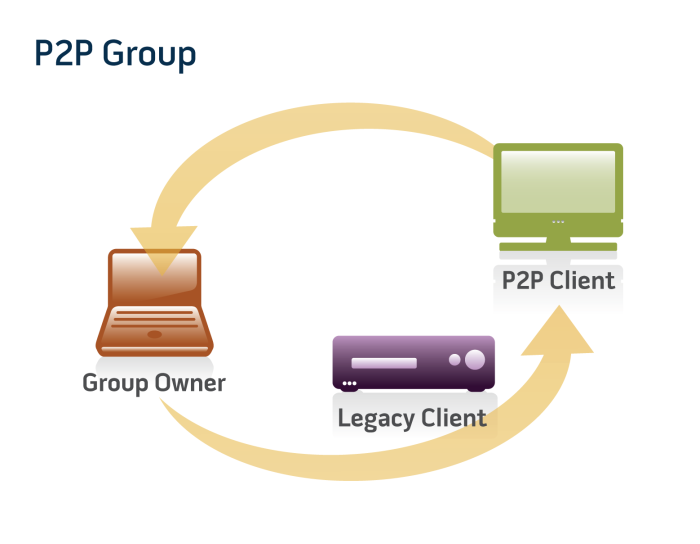
\includegraphics[width=0.7\textwidth]{images/wifidirect.png}
	\caption{The figure shows a P2P group with a Wifi Direct client and a legacy device}
	\label{fig1}
\end{figure}
\chapter{Prototypes}
\label{cha:Prototypes}
\section{Android}
Since Android 4.0, devices with appropriate hardware are allowed to connect directly to each other over WI-FI P2P without an access point between them. Android P2P framework complies with the WI-FI Alliances' WI-FI Direct certification program. With the usage of this API you are able to discover and connect to other devices when they support WI-FI P2P.  According to documentations the advantage of WI-FI P2P beside Bluetooth or similar connection types is a fast connection across distances much longer than others. This allows applications a fast exchange of data between multiple users, which could be useful for applications such as multiplayer games, photosharing applications and in general, all applications which are relying on a fast connection between a long distance.

\section{Rasberry Pi}

\section{Windows Phone}
Microsoft included Wifi Direct in his new Windows Phone 8.1 SDK, but actually there is no good documentation or sample which describes the usage of Wifi Direct in a Windows Phone app.\\
The other option would be to use there own namespace which connects two phones directly to each other, but this requires Bluetooth and WIFI and the same app on both devices. Since this is not compatible with any other devices than Windows Phones this is not good solution. Furthermore are the devices limited to the Bluetooth range which is in fact not very long.
%!TEX root = _DaBa.tex
\chapter{Evaluation}
\label{cha:Evaluation}
This chapter will point out some difficulties that have been experienced while developing the prototypes for the car2car project.

\section{Communication between mobile platforms}
\label{sec:CommunicationBetweenPlattforms}
One big problem is the compatibility between mobile platforms. The goal was to cover as many platforms as possible. For this project Windows Phone and Android was chosen. iOS was considered at the beginning too, however it uses a proprietary protocol, which is not compatible with other platforms and therefore can only be used for iOS devices. Problems occured with Windows Phone too. According to the Windows Phone documentation, it should be possible to connect with other platforms. However there are no good sample implementation for accomplishing this goal. In general the wifi direct technology is not mature on Windows Phone. Only Android could satisfy the needs. An implementation of a wifi direct prototype could be accomplished and a connection with a Raspberry pi could be generated.

\section{Wifi direct}
\label{sec:WifiDirect}
The field study of wifi direct is very new. In case of the Raspberry Pi prototype, there were not much sources to gather information on how to setup a wifi direct connection successfully. Even the Realtek P2P UI console application did not work reliably. For Android wifi direct is supported since Android 4.0. However the hardware manufacturer have the final say to enable this feature. 


%!TEX root = _DaBa.tex
\chapter{Conclusion and future work}
\label{cha:ConclusionFutureWork}
This chapter will recap on the goals of this paper and will present future work and changes in the field of C2C communication.

\section{Conclusion}
\label{sec:Conclusion}
As a conclusion it can be said, that wifi direct is at the moment not the ideal solution to bring C2C communication to the public. The problem is, that most manufacturers have their own protocol for this technologie. iOS has the MultiPeerFramework, which can be used only for iOS Devices. Windows Phone introduced Wifi direct within the Windows Phone 8.1 SDK release, which is at the moment only available for developers, however no suitable documentation was found. Android has introduced Wifi direct since Android 4.0 and obviously uses the standard protocol, because a connection could be established between the Raspberry Pi and an Android Device. Speaking of the Rapsberry Pi the current implementation for supporting wifi direct is not reliable enough at the moment to be used in such field as C2C communication. In some tests the connection was aborted all of a sudden. This technologie needs to be more mature and consistent protocols or implementations among the smartphone manufacturers are needed.

\section{Future work}
\label{sec:FutureWork}
If the implementation of the prototype will be continued, the next step would be to concentrate on the Raspberry Pi platform. Further tests should be processed and a deeper investigation of the wifi direct/P2P protocol would be necessary. If wifi direct will not become more reliable in the future, it would be possible to use a different technologie, like communication over light. Breaking lights could be used, however it depends on free sight to the lights of the car in front and at the back. At the moment the prototype implementation is able to communicate with one device, later it should be possible to broadcast messages and information to more than one device in the near surroundings. Recent news show that C2C communication will be more and more important for the information technologie. INTEL for example, recently launched the automotive platform "Kendrick Peak", which should be used in in-vehicle-infotainment systems, based on an embedded atom chipset. This platform could be used in the field of C2C communication too. At the moment INTEL works with car manufacturers like BMW, Jaguar, Landrover, Kia and Hyundai on this platform. A cheap and interesting solution for C2C communication could be the "Vehicle Pi"\footnote{http://vehiclepi.com/}. It is a shield specially designed for the Raspberry Pi, which offers sensors and interfaces that can be connected to the car and retrieve information from it. 


%%%----------------------------------------------------------

\addcontentsline{toc}{chapter}{Listings}
%\lstlistoflistings
\listoffigures


%%%----------------------------------------------------------
\MakeBibliography
%%%----------------------------------------------------------

\end{document}
